\documentclass{article}
\usepackage{fancyhdr}
\usepackage{geometry}
\usepackage{amsfonts}
\usepackage{amsthm}
\usepackage{tikz} % Add this line to include tikz package

% Set page margins
\geometry{margin=1in}

% Define fancy header
\pagestyle{fancy}
\fancyhf{}
\renewcommand{\headrulewidth}{0.4pt}
\fancyhead[L]{Patrick Brown}
\fancyhead[C]{Optimization - Homework 1}
\fancyhead[R]{\thepage}

% Define a new environment for answers
\newenvironment{answer}
    {\par\noindent\textbf{Answer:}\par}
    {\par}

\begin{document}

\begin{center}
\Large\textbf{The University of Texas at Austin}\\[0.5em]
\large\textbf{Optimization}\\[0.5em]
\large\textbf{Homework 1}
\end{center}

\vspace{1em}

\textbf{Instructors:} Constantine Caramanis, Sujay Sanghavi

\vspace{1em}

\textbf{Submitting solutions:} Please submit your solutions as a single pdf file. If you have code or figures, please include these in the pdf.

\section{Convex Sets, Convex Functions, Preservation of Convexity}

\begin{enumerate}
    \item 
    \begin{enumerate}
        \item 
        \begin{answer}
        To show that the intersection of convex sets is convex, we will prove that the intersection of any finite number of convex sets is convex. Let $\{C_i\}_{i=1}^n$ be a collection of convex sets, and let $C = \bigcap_{i=1}^n C_i$ be their intersection.

        1) First, we need to show that $C$ is non-empty. This is assumed implicitly, as the intersection of convex sets can be empty (e.g., two disjoint convex sets).

        2) Let $\mathbf{x}, \mathbf{y} \in C$. This means $\mathbf{x}, \mathbf{y} \in C_i$ for all $i = 1, 2, ..., n$.

        3) To prove $C$ is convex, we need to show that for any $\lambda \in [0,1]$, the point $\mathbf{z} = \lambda\mathbf{x} + (1-\lambda)\mathbf{y}$ is also in $C$.

        4) For each $C_i$:
           - Since $C_i$ is convex and $\mathbf{x}, \mathbf{y} \in C_i$, we know that $\mathbf{z} = \lambda\mathbf{x} + (1-\lambda)\mathbf{y} \in C_i$ for any $\lambda \in [0,1]$.

        5) Since $\mathbf{z} \in C_i$ for all $i = 1, 2, ..., n$, we can conclude that $\mathbf{z} \in \bigcap_{i=1}^n C_i = C$.

        6) Therefore, for any two points in $C$ and any $\lambda \in [0,1]$, the convex combination of these points is also in $C$.

        This satisfies the definition of a convex set, proving that $C$ is convex. Thus, the intersection of any finite number of convex sets is convex.

        Note: This proof can be extended to the intersection of an infinite number of convex sets by considering arbitrary subsets of the intersection and applying the same logic.
        \end{answer}

        \item 
        \begin{answer}
        An example where the union of two convex sets is not convex:
        
        Consider two disjoint circles in $\mathbb{R}^2$. Each circle is a convex set, but their union is not convex because a line segment connecting a point in one circle to a point in the other circle would not be entirely contained within the union.
        
        \begin{center}
        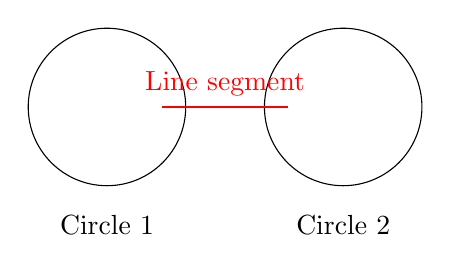
\begin{tikzpicture}
            % Draw two circles
            \draw (0,0) circle (1cm);
            \draw (3,0) circle (1cm);
            
            % Draw a line segment between the circles
            \draw[red, thick] (0.7,0) -- (2.3,0);
            
            % Add labels
            \node at (0,-1.5) {Circle 1};
            \node at (3,-1.5) {Circle 2};
            \node[red] at (1.5,0.3) {Line segment};
        \end{tikzpicture}
        \end{center}
        
        As shown in the figure, the red line segment connecting points in the two circles is not entirely contained within the union of the circles, demonstrating that the union is not convex.
        \end{answer}

        \item 
        \begin{answer}
        To show that the maximum of convex functions is convex, let $f_1$ and $f_2$ be convex functions, and $f_{\max}(x) = \max\{f_1(x), f_2(x)\}$.
        
        For any $\mathbf{x}, \mathbf{y}$ and $\lambda \in [0,1]$:
        
        $f_{\max}(\lambda\mathbf{x} + (1-\lambda)\mathbf{y})$
        $= \max\{f_1(\lambda\mathbf{x} + (1-\lambda)\mathbf{y}), f_2(\lambda\mathbf{x} + (1-\lambda)\mathbf{y})\}$
        
        $\leq \max\{\lambda f_1(\mathbf{x}) + (1-\lambda)f_1(\mathbf{y}), \lambda f_2(\mathbf{x}) + (1-\lambda)f_2(\mathbf{y})\}$
        
        $\leq \lambda \max\{f_1(\mathbf{x}), f_2(\mathbf{x})\} + (1-\lambda) \max\{f_1(\mathbf{y}), f_2(\mathbf{y})\}$
        
        $= \lambda f_{\max}(\mathbf{x}) + (1-\lambda) f_{\max}(\mathbf{y})$
        
        This proves that $f_{\max}$ satisfies the definition of convexity, and thus the maximum of convex functions is convex.
        \end{answer}
    \end{enumerate}

    \section{More Convex Sets, Convex Functions, Preservation of Convexity}

\begin{enumerate}
    \item 
    \begin{enumerate}
        \item 
        \begin{answer}
        An example where the minimum of two convex functions is not convex:
        
        Consider $f_1(x) = x^2$ and $f_2(x) = (x-2)^2$. Both are convex functions.
        Let $f_{\min}(x) = \min\{f_1(x), f_2(x)\}$.
        
        $f_{\min}(x)$ is not convex because it forms a "V" shape with a non-convex kink at $x=1$, where the two parabolas intersect.

        \begin{center}
        \begin{tikzpicture}[scale=1.2]
            % Draw axes
            \draw[->] (-1,0) -- (3,0) node[right] {$x$};
            \draw[->] (0,0) -- (0,4) node[above] {$y$};
            
            % Draw f1(x) = x^2
            \draw[blue, domain=-1:3, samples=100] plot (\x, {\x*\x}) node[right] {$f_1(x)$};
            
            % Draw f2(x) = (x-2)^2
            \draw[red, domain=-1:3, samples=100] plot (\x, {(\x-2)*(\x-2)}) node[right] {$f_2(x)$};
            
            % Draw f_min(x)
            \draw[green, thick, domain=-1:1, samples=100] plot (\x, {\x*\x});
            \draw[green, thick, domain=1:3, samples=100] plot (\x, {(\x-2)*(\x-2)});
            
            % Label f_min(x)
            \node[green] at (2.5,1.5) {$f_{\min}(x)$};
            
            % Mark the non-convex kink
            \fill[black] (1,1) circle (2pt);
            \node[below right] at (1,1) {kink};
            
            % Label axes
            \node[below left] at (0,0) {$0$};
            \node[below] at (2,0) {$2$};
        \end{tikzpicture}
        \end{center}
        
        As shown in the figure, $f_{\min}(x)$ (in green) follows $f_1(x)$ for $x < 1$ and $f_2(x)$ for $x > 1$, creating a non-convex kink at $x=1$. This demonstrates that the minimum of two convex functions is not necessarily convex.
        \end{answer}

        \item 
        \begin{answer}
        An example of two closed convex sets that are disjoint but cannot be strictly separated:
        
        Consider in $\mathbb{R}^2$:
        $C_1 = \{(x,y) : y \geq e^x\}$
        $C_2 = \{(x,y) : y \leq 0\}$
        
        These sets are closed, convex, and disjoint. However, they cannot be strictly separated because for any separating hyperplane (in this case, a line), there will always be points from both sets arbitrarily close to the hyperplane as $x \to -\infty$.
        \end{answer}

        \item 
        \begin{answer}
        To show that any sub-level set of a convex function is convex:
        
        Let $f$ be a convex function and $L_c = \{x : f(x) \leq c\}$ be a sub-level set.
        Take any $x_1, x_2 \in L_c$ and $\lambda \in [0,1]$.
        
        $f(\lambda x_1 + (1-\lambda)x_2) \leq \lambda f(x_1) + (1-\lambda)f(x_2)$ (by convexity of $f$)
        $\leq \lambda c + (1-\lambda)c = c$
        
        Therefore, $\lambda x_1 + (1-\lambda)x_2 \in L_c$, proving $L_c$ is convex.
        
        Example of a non-convex function with convex sub-level sets:
        
        Consider $f(x) = -x^2$. This function is concave (thus not convex), but all its sub-level sets are convex intervals. For any $c$, $L_c = \{x : -x^2 \leq c\} = [-\sqrt{-c}, \sqrt{-c}]$, which is a convex set.
        \end{answer}
    \end{enumerate}
\end{enumerate}


\end{enumerate}

\section{Half-Space Representation of Points Closer to v1 than v2}

\begin{enumerate}
    \item Two dimensions:
    \begin{answer}
    For $v_1 = (-1, 0)^T$ and $v_2 = (1, 0)^T$, the set of points closer to $v_1$ than $v_2$ forms a half-space. This half-space is the left half of the plane, separated by the vertical line x = 0. The shaded region would be all points with x < 0.
    \end{answer}

    \item Finding c and d for the two-dimensional case:
    \begin{answer}
    For the given example, we need to find $c = (c_1, c_2)^T$ and $d \in \mathbb{R}$ such that:
    
    $\{(x_1, x_2)^T : c_1x_1 + c_2x_2 \leq d\}$
    
    represents the shaded region (x < 0).
    
    We can choose:
    $c = (1, 0)^T$ and $d = 0$
    
    This gives us the inequality: $x_1 \leq 0$, which correctly describes the left half-plane.
    \end{answer}

    \item Generalization to n dimensions:
    \begin{answer}
    For general points $v_1, v_2 \in \mathbb{R}^n$, we can find $c \in \mathbb{R}^n$ and $d \in \mathbb{R}$ as follows:
    
    $c = v_2 - v_1$
    $d = \frac{1}{2}(||v_2||^2 - ||v_1||^2)$
    
    To prove this, we start with the condition $||x - v_1||_2 \leq ||x - v_2||_2$:
    
    $(x - v_1)^T(x - v_1) \leq (x - v_2)^T(x - v_2)$
    
    Expanding and simplifying:
    
    $x^Tx - 2v_1^Tx + v_1^Tv_1 \leq x^Tx - 2v_2^Tx + v_2^Tv_2$
    
    $-2v_1^Tx + v_1^Tv_1 \leq -2v_2^Tx + v_2^Tv_2$
    
    $2(v_2 - v_1)^Tx \leq v_2^Tv_2 - v_1^Tv_1$
    
    $(v_2 - v_1)^Tx \leq \frac{1}{2}(v_2^Tv_2 - v_1^Tv_1)$
    
    This is equivalent to $c^Tx \leq d$ with $c$ and $d$ as defined above.
    
    Thus, we have shown that the set of points in $\mathbb{R}^n$ that are closer to point $v_1$ than to point $v_2$ indeed form a half-space, represented by $\{x : c^Tx \leq d\}$.
    \end{answer}
\end{enumerate}

\end{document}